\documentclass[12pt, varwidth, border=5mm]{standalone}
\usepackage{tikz}
\usepackage{amsmath}
% Underlining package
\usepackage{ulem}
\usetikzlibrary{calc}
\usetikzlibrary{angles,quotes}
% \usepackage[a4paper, portrait, margin=1cm]{geometry}

\begin{document}
\section*{ }
    \begin{minipage}{0.55\textwidth}
  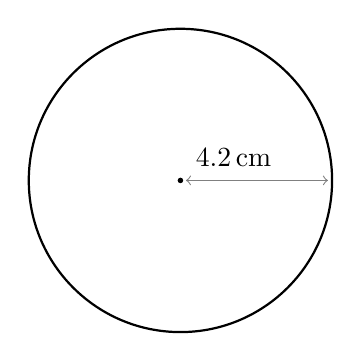
\begin{tikzpicture}[scale=1.0, baseline=(current bounding box.north)]
    \begin{scope}[rotate=0]
        \coordinate (A) at (0,0);
        % Define B using polar coordinates from A
        \coordinate (B) at ($(A) + (0:1.926)$);
        \fill (A) circle(1pt);
        \draw[thick] (A) circle (1.926);
        \draw[<->, gray, shorten <=2pt, shorten >=1.5pt]
          (A) -- (B)
          node[pos=0.35, sloped, above, fill=white, inner sep=2pt, xshift=0pt, yshift=3pt, transform shape]
          {\textcolor{black}{$4.2\,\text{cm}$}};
    \end{scope}
  \end{tikzpicture}
\end{minipage}%
\hfill
\begin{minipage}{.4\textwidth}
  \begin{align*}
  \text{Area} &= \pi r^2 \\
  \text{Area} &= \pi \times (\dotuline{~~~~~~~~~~~~}\,\text{cm})^2 \\
  \text{Area} &\approx \dotuline{~~~~~~~~~~~~} \,\text{cm}^2
  \end{align*}
\end{minipage}

\end{document}
